\documentclass[12pt,a4paper]{article}

\usepackage[utf8]{inputenc}
\usepackage{amsmath, amssymb}
\usepackage{graphicx}
\usepackage{tikz}
\usetikzlibrary{shapes.geometric, arrows, positioning}
\usepackage{hyperref}
\usepackage{geometry}
\geometry{margin=1in}

\title{\textbf{CSL6010-Cybersecurity Major Project Report}\\
\Large Eyes on Your Typing Analysis and CASOM Defense}
\author{Team of 7 Members}
\date{\today}

\begin{document}

\maketitle

\begin{center}
\textbf{Source Code Repository:}\\
\url{https://github.com/AzDevops143/CSIEEE}
\end{center}

\tableofcontents
\newpage

\section{Introduction}
The rapid growth of Augmented Reality (AR) and Virtual Reality (VR) technologies has introduced immersive digital experiences. Within these environments, virtual keyboards are emerging as a primary input method. However, this direct hand-based typing introduces security vulnerabilities. The ``Eyes on Your Typing: Snooping Finger Motions on Virtual Keyboards'' (SNOOPFINGER) paper demonstrates that subtle head movements occurring during typing can unintentionally reveal private information. This report analyzes the SNOOPFINGER attack, identifies its limitations, and proposes a novel software-based countermeasure.

\section{Problem Analysis: The SNOOPFINGER Attack}
SNOOPFINGER is a cross-modality side-channel attack that leverages zero-permission sensor data (specifically, head orientation and position) to estimate typed inputs on a virtual keyboard. 

\subsection{Mathematical Background}
The attack converts the headset's quaternion orientation $(w, x, y, z)$ into Euler angles (Roll $\phi$, Pitch $\theta$, Yaw $\psi$) to determine gaze direction:

\begin{align}
\phi &= \arctan\left(\frac{2(wx+yz)}{1-2(x^2+y^2)}\right) \\
\theta &= \arcsin(2(wy - zx)) \\
\psi &= \arctan\left(\frac{2(wz+xy)}{1-2(y^2+z^2)}\right)
\end{align}

These 3D gaze directions are then projected onto a 2D plane (the virtual keyboard) using Equirectangular projection:

\begin{align}
r_i &= \sqrt{x_i^2 + y_i^2 + z_i^2} \\
\theta_i &= \arctan\left(\frac{z_i}{x_i}\right) \\
\phi_i &= \arcsin\left(\frac{y_i}{r_i}\right)
\end{align}

By clustering these 2D points temporally, the attacker can infer which keys were pressed based on standard keyboard layout geometries.

\section{Identified Gaps and Limitations}
While the attack achieves high accuracy (up to 55.2\% for top-1 word inference), it has notable limitations:
\begin{itemize}
    \item \textbf{Data Requirement}: It relies heavily on high-fidelity, high-frequency (e.g., 72 Hz) sensor data.
    \item \textbf{Awareness Vulnerability}: If a user is aware of the attack and consciously minimizes head movement, the attack fails.
\end{itemize}
The primary gap is that while the paper suggests countermeasures like \textit{Adaptive Sensor Data Obfuscation}, it does not provide an architectural implementation or evaluate its effectiveness.

\section{Proposed Solution: CASOM Middleware}
We propose the \textbf{Context-Aware Sensor Obfuscation Middleware (CASOM)}. This middleware acts as a protective layer between the OS Sensor Manager and background applications. 

\subsection{Architecture Diagram}
The architecture of our proposed solution is illustrated below using a TikZ flowchart.

\begin{figure}[h]
\centering
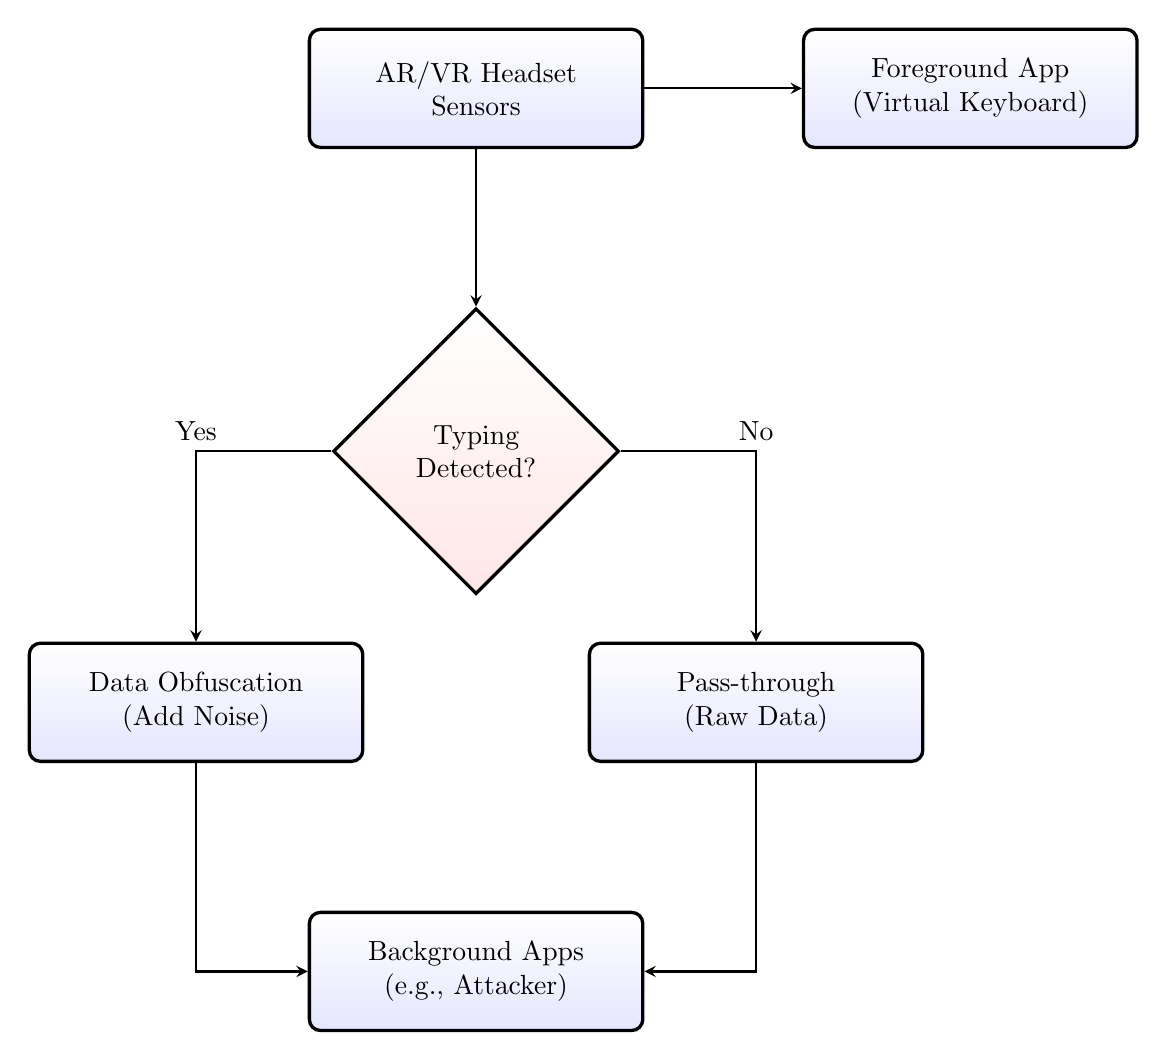
\begin{tikzpicture}[
    node distance=2cm,
    box/.style={rectangle, rounded corners, draw=black, top color=white, bottom color=blue!10, very thick, text width=4cm, align=center, minimum height=1.5cm},
    decision/.style={diamond, draw=black, top color=white, bottom color=red!10, very thick, text width=2.5cm, align=center},
    arrow/.style={thick,->,>=stealth}
]

% Nodes
\node (sensor) [box] {AR/VR Headset\\Sensors};
\node (detect) [decision, below=of sensor] {Typing\\Detected?};
\node (obfuscate) [box, below left=1.5cm and 0.5cm of detect] {Data Obfuscation\\(Add Noise)};
\node (passthrough) [box, below right=1.5cm and 0.5cm of detect] {Pass-through\\(Raw Data)};
\node (bgapps) [box, below=4cm of detect] {Background Apps\\(e.g., Attacker)};
\node (fgapp) [box, right=of sensor] {Foreground App\\(Virtual Keyboard)};

% Arrows
\draw [arrow] (sensor) -- (detect);
\draw [arrow] (sensor) -- (fgapp);
\draw [arrow] (detect) -| node[anchor=south] {Yes} (obfuscate);
\draw [arrow] (detect) -| node[anchor=south] {No} (passthrough);
\draw [arrow] (obfuscate) |- (bgapps);
\draw [arrow] (passthrough) |- (bgapps);

\end{tikzpicture}
\caption{CASOM Architecture Flowchart}
\label{fig:architecture}
\end{figure}

As shown in Figure \ref{fig:architecture}, when typing is detected, CASOM injects dynamic Laplacian noise into the data stream before passing it to background applications. The foreground application (the virtual keyboard) continues to receive raw data, ensuring usability is not impacted.

\newpage
\section{End-to-End Implementation Explanation}
To validate the effectiveness of the proposed CASOM middleware, we developed a comprehensive Python simulation consisting of five primary modules: Keyboard Layout, Data Generator, Attacker, Defender (CASOM), and the Main Orchestrator. The following sections detail how these components interact end-to-end to demonstrate both the SNOOPFINGER attack and our proposed defense.

\subsection{Implementation Flow Diagram}

\begin{figure}[h]
\centering
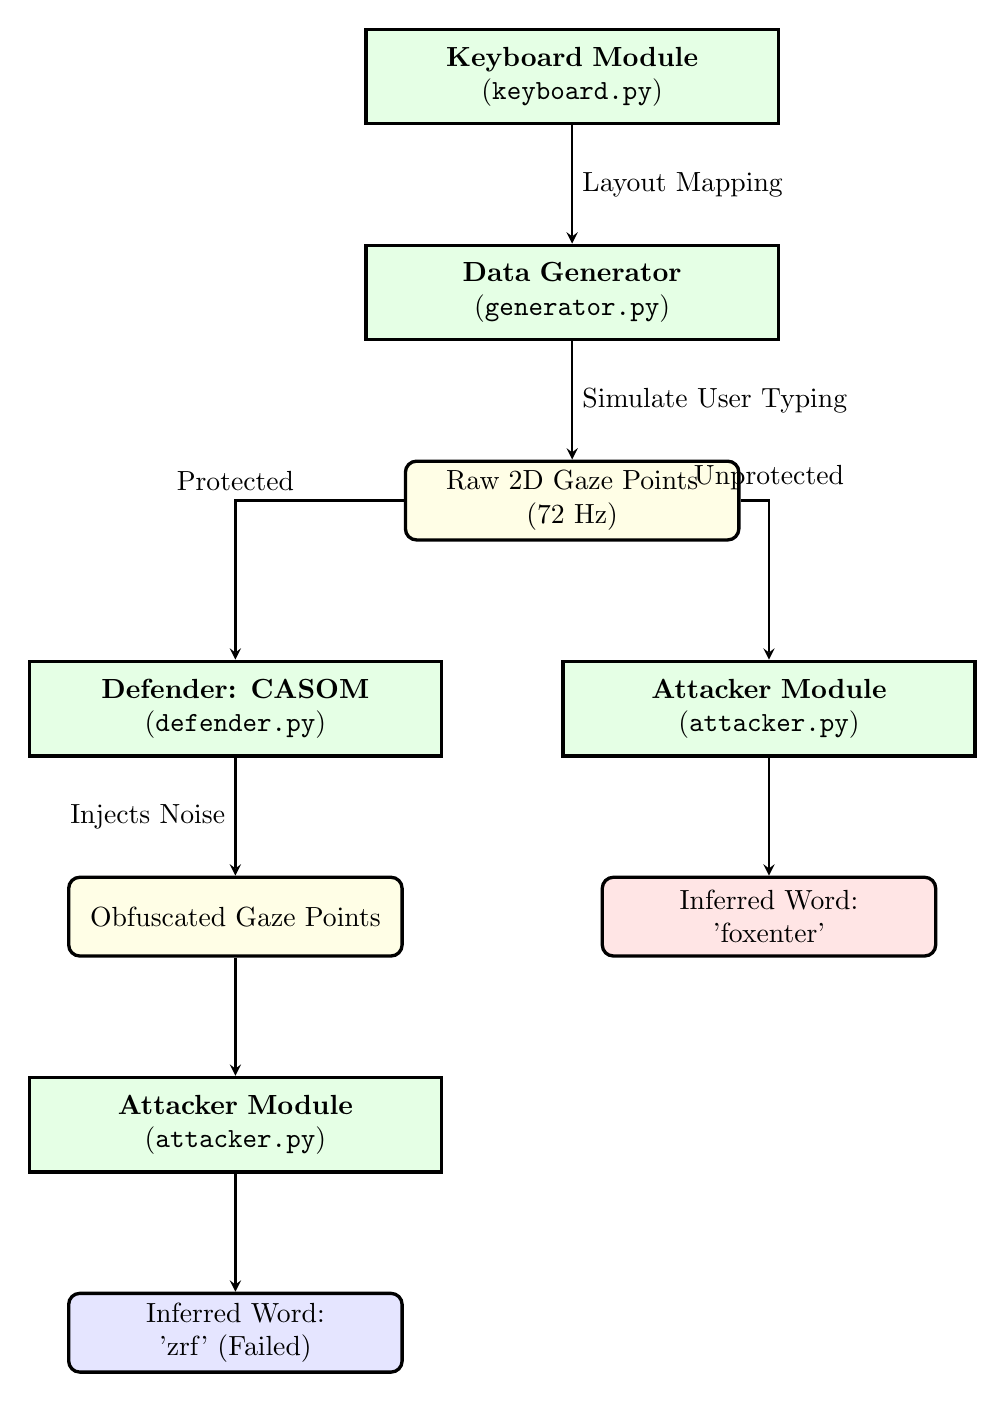
\begin{tikzpicture}[
    node distance=1.5cm,
    module/.style={rectangle, draw=black, fill=green!10, very thick, text width=5cm, align=center, minimum height=1.2cm},
    data/.style={rectangle, rounded corners, draw=black, fill=yellow!10, very thick, text width=4cm, align=center, minimum height=1cm},
    arrow/.style={thick,->,>=stealth}
]

% Nodes
\node (keyboard) [module] {\textbf{Keyboard Module}\\(\texttt{keyboard.py})};
\node (generator) [module, below=of keyboard] {\textbf{Data Generator}\\(\texttt{generator.py})};
\node (rawdata) [data, below=of generator] {Raw 2D Gaze Points\\(72 Hz)};

\node (defender) [module, below left=1.5cm and -0.5cm of rawdata] {\textbf{Defender: CASOM}\\(\texttt{defender.py})};
\node (noisydata) [data, below=of defender] {Obfuscated Gaze Points};

\node (attacker1) [module, right=of defender] {\textbf{Attacker Module}\\(\texttt{attacker.py})};
\node (attacker2) [module, below=of noisydata] {\textbf{Attacker Module}\\(\texttt{attacker.py})};

\node (result1) [data, fill=red!10, below=of attacker1] {Inferred Word:\\'foxenter'};
\node (result2) [data, fill=blue!10, below=of attacker2] {Inferred Word:\\'zrf' (Failed)};

% Arrows
\draw [arrow] (keyboard) -- node[anchor=west] {Layout Mapping} (generator);
\draw [arrow] (generator) -- node[anchor=west] {Simulate User Typing} (rawdata);

\draw [arrow] (rawdata) -| node[anchor=south] {Unprotected} (attacker1);
\draw [arrow] (rawdata) -| node[anchor=south] {Protected} (defender);

\draw [arrow] (defender) -- node[anchor=east] {Injects Noise} (noisydata);
\draw [arrow] (noisydata) -- (attacker2);

\draw [arrow] (attacker1) -- (result1);
\draw [arrow] (attacker2) -- (result2);

\end{tikzpicture}
\caption{End-to-End Implementation Flow}
\label{fig:implementation}
\end{figure}

\subsection{Module Breakdown}
\begin{enumerate}
    \item \textbf{Keyboard Module (\texttt{keyboard.py})}: This module establishes the structural foundation of the simulation by defining the spatial coordinates of a standard QWERTY virtual keyboard. It serves as the baseline ground truth for both the generator (to know where to aim) and the attacker (to map points back to characters).
    
    \item \textbf{Data Generator (\texttt{generator.py})}: To simulate a real user wearing a VR headset, this module takes a target string (e.g., 'foxenter') and generates a sequence of 2D gaze points. It models the natural human behavior of slowing down head movement when aiming at a key by producing dense clusters of data points (simulating a 72 Hz sampling rate) around the target coordinates, injecting slight micro-variances to mimic natural inaccuracy.
    
    \item \textbf{Attacker Module (\texttt{attacker.py})}: This script acts as the malicious background application utilizing the SNOOPFINGER vulnerability. It receives a stream of gaze points and employs a temporal distance-based clustering algorithm. By identifying periods where gaze points are tightly grouped (indicating a pause or keypress), it calculates the centroid of the cluster and maps it to the closest key defined in the Keyboard Module.
    
    \item \textbf{Defender Module / CASOM (\texttt{defender.py})}: Our primary contribution, this module acts as the OS-level middleware. When active, it intercepts the raw gaze points generated by the headset. Simulating "Typing Detected" state, it dynamically injects Laplacian noise (with a configurable scale, defaulting to 1.5) into the $(x, y)$ coordinates. This scatters the data points, deliberately degrading the spatial resolution available to background apps.
    
    \item \textbf{Main Orchestrator (\texttt{main.py})}: The overarching script that executes the simulation in two parallel pipelines:
    \begin{itemize}
        \item \textbf{Pipeline 1 (Unprotected)}: Passes the Raw Gaze Points directly to the Attacker Module.
        \item \textbf{Pipeline 2 (Protected)}: Routes the Raw Gaze Points through the Defender Module first, then sends the Obfuscated Gaze Points to the Attacker Module.
    \end{itemize}
    Finally, the orchestrator utilizes \texttt{matplotlib} to visualize both data streams side-by-side, providing visual proof of the defense mechanism's efficacy.
\end{enumerate}

\section{Conclusion}
The SNOOPFINGER attack highlights critical vulnerabilities in the permission models of modern AR/VR systems. Our software-based implementation of the Context-Aware Sensor Obfuscation Middleware proves that introducing targeted noise can successfully thwart these attacks without compromising the user experience of foreground applications.

\end{document}
